% !TeX root = ../main.tex

\chapter{真实决策控制任务中的样本效率及安全性提升}\label{chap:greenhouse}

为了进一步验证本论文中所提出的DPER算法和MBDP算法在强化学习样本效率及安全性方面的提升效果,我们在更复杂的真实任务中进行了实验验证。

\section{自动化温室决策控制任务}

现有的人工智能农业应用大部分还停留在基于规则的判断方法上,或是基于模拟器的搜索方法。强化学习作为一类能够自我探索和利用的弱监督算法,在生成智能决策策略上理应更适合这类复杂的工作。然而强化学习的两大难点便是算法的样本利用效率和所学策略的安全性。我们所提出的DPER算法能大幅改善样本利用效率,MBDP算法则能在不损失样本效率的前提下尽可能提升算法鲁棒性,从而间接提升所学策略的决策安全性。因此,我们考虑将本论文提出的两种算法相结合,并将其应用于真实样本极度稀缺、安全性要求高的自动化温室决策控制任务中,验证算法所带来的提升效果。

\section{算法框架与设计}

\begin{figure}[t]
\centering
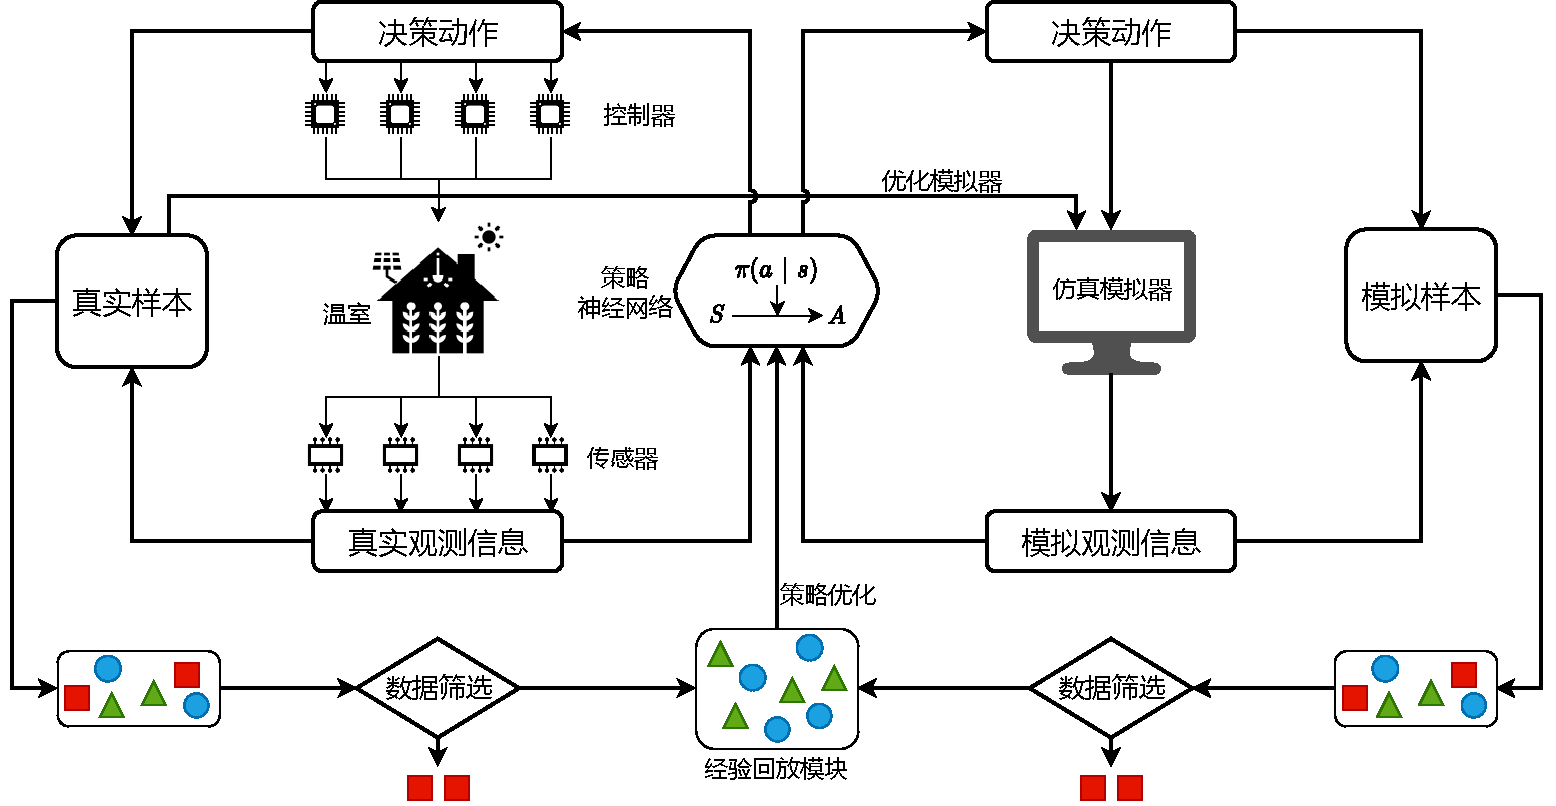
\includegraphics[width=\textwidth]{figures/framework.pdf}
\caption{自动化温室决策学习算法框架}
\label{fig:framework}
\end{figure}

我们设计了如图~\ref{fig:framework}~所示的算法框架。这个用于温室自动化的模块化框架主要由温室环境、作物生长模拟器和一个带有经验回放模块+模拟数据筛选模块的强化学习算法组成。核心部分是中央决策模块,它接收观测结果以决定下一步行动。强化学习算法则使用样本来不断优化策略。这三个部分在一个循环中交替进行,最终学到兼具样本效率和安全性的自动种植策略。算法的流程描述如算法~\ref{algo:acml-method}所示。

\begin{algorithm}[t]
\caption{Dropout模块函数}
\begin{algorithmic}
\STATE 函数 Dropout($\mathcal{B}$, $p$):
    \STATE 计算缓存$\mathcal{B}$中样本奖励的$p$-百分位: $r_p(\mathcal{B})$\\
    \FOR{$x\in \mathcal{B}$}
        \IF{$r(x)\leq r_p(\mathcal{B})$}
            \STATE 将样本 $x$ 填入 $\mathcal{B}_{\mathrm{drop}}$
        \ENDIF
    \ENDFOR
    \STATE Return $\mathcal{B}_{\mathrm{drop}}$
\end{algorithmic}
\end{algorithm}

\begin{algorithm}[t]
\caption{自动化温室决策学习算法}
\begin{algorithmic}
\STATE 初始化超参数、 策略 $\pi_\theta$、环境样本池 $\mathcal{D}_{\mathrm{real}}$、模拟样本池 $\mathcal{D}_{\mathrm{sim}}$\\
\FOR{$N_\mathrm{epoch}$ 迭代次数}
    \STATE 使用策略 $\pi_\theta$在温室中交互采取行动\\
    \STATE 将生成的样本填入 $\mathcal{D}_{\mathrm{real}}$中\\
    \STATE 将$\mathcal{D}_{\mathrm{real}}$ 分割为 $\left\{\mathcal{D}_{\mathrm{1}}, \mathcal{D}_{\mathrm{2}}, \ldots, \mathcal{D}_{\mathrm{N}}\right\}$\\
    \FOR{$N_\mathrm{train}$ 迭代次数}
        \STATE 加载预训练模型并在 $\left\{\mathcal{D}_{\mathrm{1}}, \mathcal{D}_{\mathrm{2}}, \ldots, \mathcal{D}_{\mathrm{N}}\right\}$上进行训练\\
        \STATE 得到训练后的模型集成 $\mathcal{M} = \{\mathcal{M}_{\phi_1},\mathcal{M}_{\phi_2},\ldots,\mathcal{M}_{\phi_{N}}\}$\\
        \FOR{$t=1,2,\ldots ,T$}
            \STATE 在$\mathcal{M}$ 中以概率 $\mathrm{Pr}\{\mathcal{M}_t=\mathcal{M}_{\phi_i}\mid i\sim P_{\mathcal{M}}, i\in\{1,2,\ldots,N\}\}$挑选模型$\mathcal{M}_t$\\
            \STATE 使用策略$\pi_\theta$在模型$\mathcal{M}_t$上交互产生样本$x=\left(s_{t+1},s_t,a_t\right)$ \\
            \STATE 将样本填入 $\mathcal{B}^{\pi_\theta,\mathcal{M}}$\\
        \ENDFOR
        \STATE $\mathcal{B}^{\pi_\theta,\mathcal{M}}_p$ = Dropout($\mathcal{B}^{\pi_\theta,\mathcal{M}}$, $p$)
        \STATE 将 $\mathcal{B}^{\pi,\mathcal{M}^\alpha}_p$ 中的数据填入 $\mathcal{D}_\mathrm{sim}$
    \ENDFOR
    \STATE $\mathcal{B}^{\pi_\theta}_p$ = Dropout($\mathcal{D}_{\mathrm{real}}$, $p$); $\mathcal{D}_{\mathrm{real}} = \mathcal{B}^{\pi_\theta}_p$\\
    \STATE 在 $\mathcal{D}_{\mathrm{sim}}$ 和 $\mathcal{D}_{\mathrm{real}}$上优化策略$\pi_\theta$ : $\theta\leftarrow \theta - \lambda\nabla_\theta V^{{\pi_\theta},\mathcal{M}}_p(\mathcal{D}_{\mathrm{sim}}; \mathcal{D}_{\mathrm{real}})$
\ENDFOR
\end{algorithmic}\label{algo:acml-method}
\end{algorithm}

\section{实验设计与结果分析}

\begin{figure}
\centering
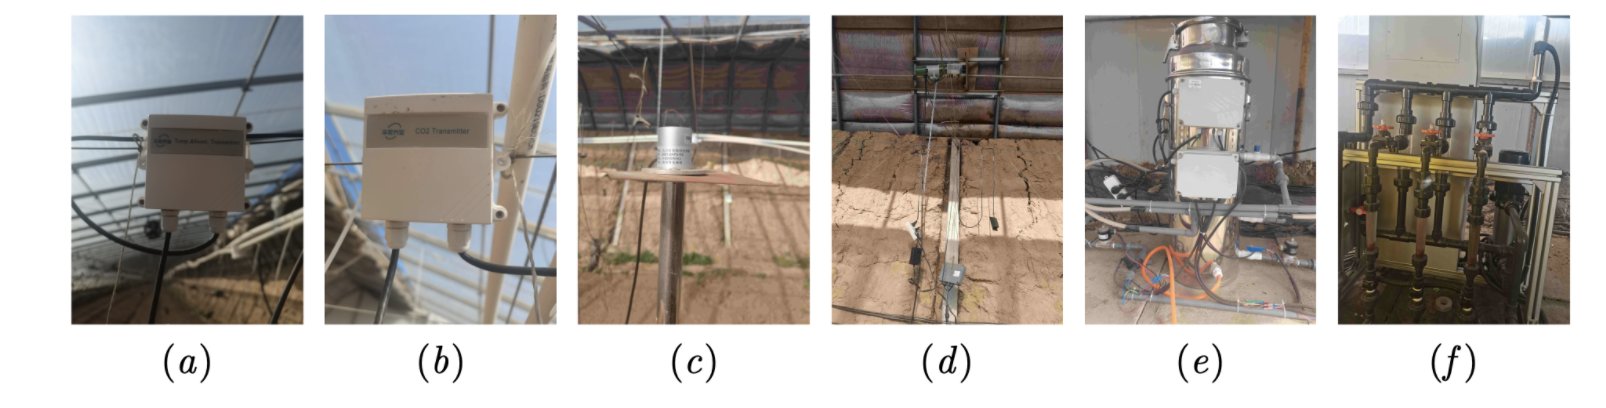
\includegraphics[width=\textwidth]{figures/devices.png}
\caption{温室自动化设备}
\label{fig:devices}
\end{figure}

我们在真实环境中部署了如图~\ref{fig:devices}所示的自动化监测与控制设备,它们的工作效果分别是:

\begin{itemize}
    \item 温度、湿度和CO$_2$传感器:在温室内悬挂多个测量盒,并对其读数进行平均取值(有时对不同位置采用不同的加权系数),以获得温度、湿度和CO$_2$的参数。
    \item PAR传感器:温室通过测量光合有效辐射来跟踪PAR参数。
    \item 通风控制器:当温室温度超过通风设定值时,通风口将被打开到一定程度,其打开角度以百分比表示。
    \item CO$_2$生成器:当CO$_2$浓度低于设定值时,CO$_2$生成器将通过管道系统供应CO$_2$。
    \item 灌溉控制器:根据相关的农作物设定值,包括灌溉时间和浇水量,自动进行滴灌灌溉。
\end{itemize}

基于上述的传感器和控制器,我们总共可以收集到22种不同种类的观测变量,构成275维的观测状态空间;并有6种可用于控制温室的动作变量,构成52维的行为动作空间。温室可观测状态信息空间的具体构成信息如表~\ref{tab:obs-space}~所示,温室可执行动作空间的具体构成如表~\ref{tab:act-space}~所示。同时,我们还设计了净利润$=$收益$-$成本来作为策略决策效果的评价指标。其中收益的计算方式为收获果实的重量$\times$单位重量的价格,成本的计算方式为电力、热力、$CO_2$和水等资源的消耗量$\times$单位资源的价格。

\begin{table}[htbp]
\centering
\caption{温室可观测状态信息空间}
\begin{tabular}{cccc|cccc}
\toprule
\textbf{属性} & \textbf{最小值} & \textbf{最大值} & \textbf{维度} & \textbf{属性} & \textbf{最小值} & \textbf{最大值} & \textbf{维度}\\
\midrule
温度  & 13           & 32           & 24           & 种植天数                                     & 0            & 365          & 1            \\
CO$_2$ 浓度                                   & 400          & 1000         & 24           & 温室温度                        & -30          & 100          & 24           \\
光照时间                                     & 0            & 24           & 1            & 温室湿度                            & 0            & 100          & 24           \\
无光照时间                                    & 0            & 24           & 1            & 温室 CO$_2$ 浓度               & 400          & 1000         & 24           \\
灌溉开始时间                             & 0            & 24           & 1            & 光照密度                   & 0            & 2000         & 24           \\
灌溉停止时间                              & 0            & 24           & 1            & 日累积灌溉量           & 0            & 10           & 1            \\
室外辐射强度                           & 0            & 2000         & 24           & 日累积排水量                & 0            & 10           & 1            \\
室外温度                               & -30          & 50           & 24           & 叶片区域                                   & 0            & 10           & 1            \\
室外湿度                                  & 0            & 100          & 24           & 当前果实数量                  & 0            & 1000         & 1            \\
风速                                        & 0            & 25           & 24           & 累积作物鲜重 & 0            & 100          & 1            \\
虚拟天空温度                           & -20          & 20           & 24           & 累积作物干重   & 0            & 100          & 1            \\
\bottomrule
\end{tabular}
\label{tab:obs-space}
\end{table}

\begin{table}[htbp]
\centering
\caption{温室可执行动作空间}
\begin{tabular}{cccc}
\toprule
\textbf{属性}                                     & \textbf{最小值} & \textbf{最大值} & \textbf{维度} \\
\midrule
温度          & 13           & 32           & 24           \\
CO$_2$ 浓度               & 400          & 1000         & 24           \\
光照时间                 & 0            & 24           & 1            \\
无光照时间                & 0            & 24           & 1            \\
灌溉开始时间         & 0            & 24           & 1            \\
灌溉停止时间          & 0            & 24           & 1            \\
\bottomrule
\end{tabular}
\label{tab:act-space}
\end{table}

\begin{figure}[t]
\centering
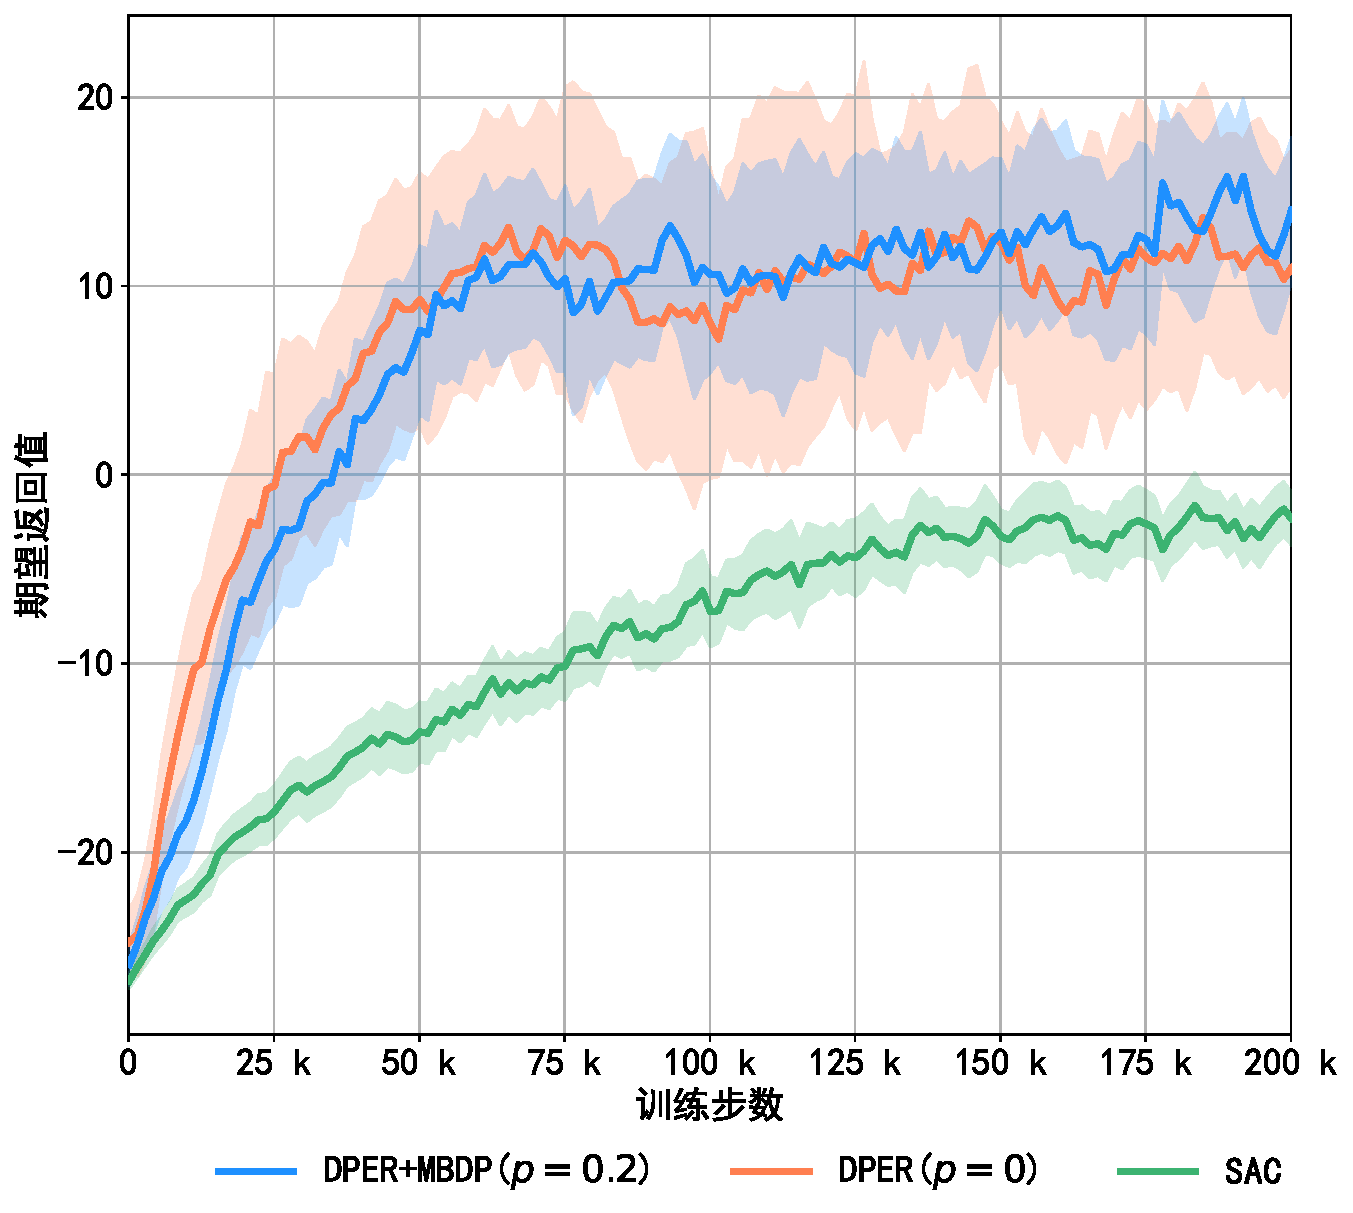
\includegraphics[width=\textwidth]{figures/acml-train.pdf}
\caption{自动温室决策学习算法的学习曲线}
\label{fig:acml-train}
\end{figure}

\begin{figure}[t]
\centering
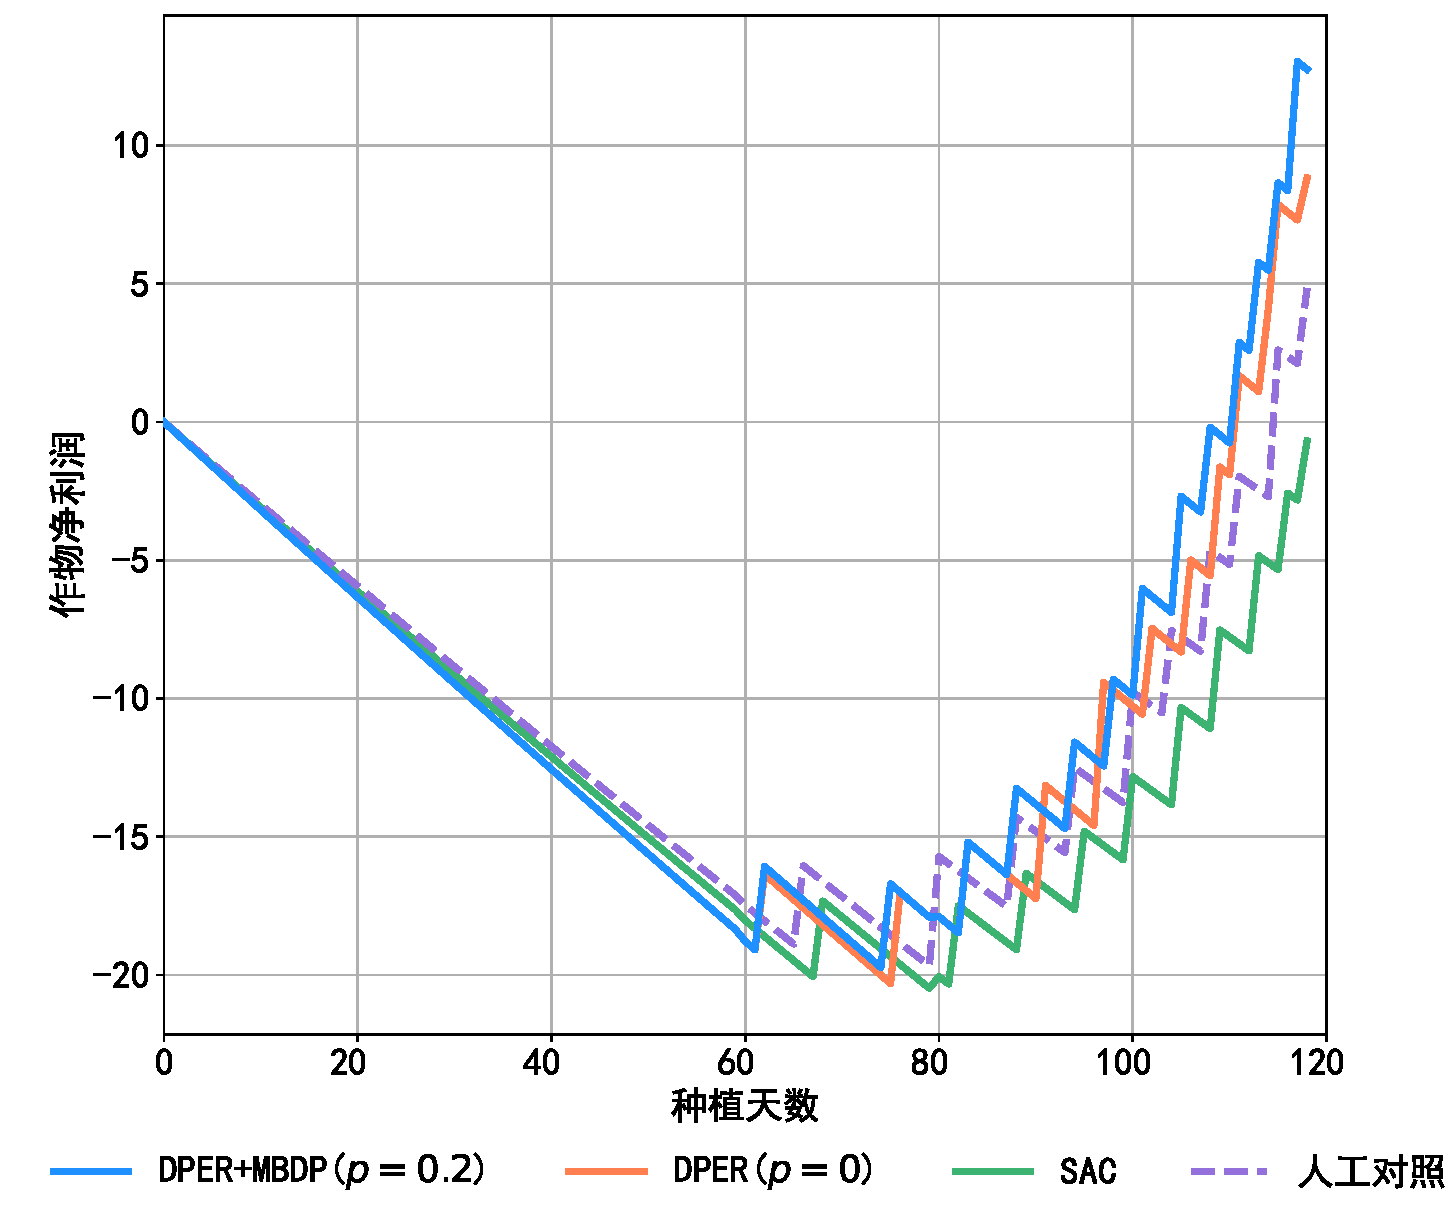
\includegraphics[width=\textwidth]{figures/acml-test.pdf}
\caption{自动温室决策学习算法的测试结果}
\label{fig:acml-test}
\end{figure}

我们训练了两种不同版本的算法,一种是有样本筛选($p=0.2$),一种是没有样本丢弃($p=0$)。此外,我们还采用了广泛使用的SAC算法作为比较的基线。在预测长度为120天的设定下,这些算法以120天的总利润作为优化目标进行训练。

如图~\ref{fig:acml-train}~左侧所示,有样本筛选的算法比没有样本晒的算法收敛效果更好,方差更小。这主要是因为样本筛选模块会丢弃一部分反馈值过高的样本,避免了局部最优。同时,智能体更关注最坏情况下的状态,所以其方差更小。至于作为基线算法的SAC算法,它的表现远比我们的算法差,这是由于无模型方法的样本效率低,使得它很难在有限的样本中学习到足够的信息。

此外,我们在温室模拟器上评估了不同算法所学习到的种植策略,~\ref{fig:acml-test}~所示,我们可以得出结论:

\begin{enumerate}
    \item 在作物未生长的早期阶段,所有的种植策略均具有相似的性能;
    \item 当作物逐渐开始收获时,我们的算法大幅优于作为对比的基线算法。
\end{enumerate}


\begin{figure}
\centering
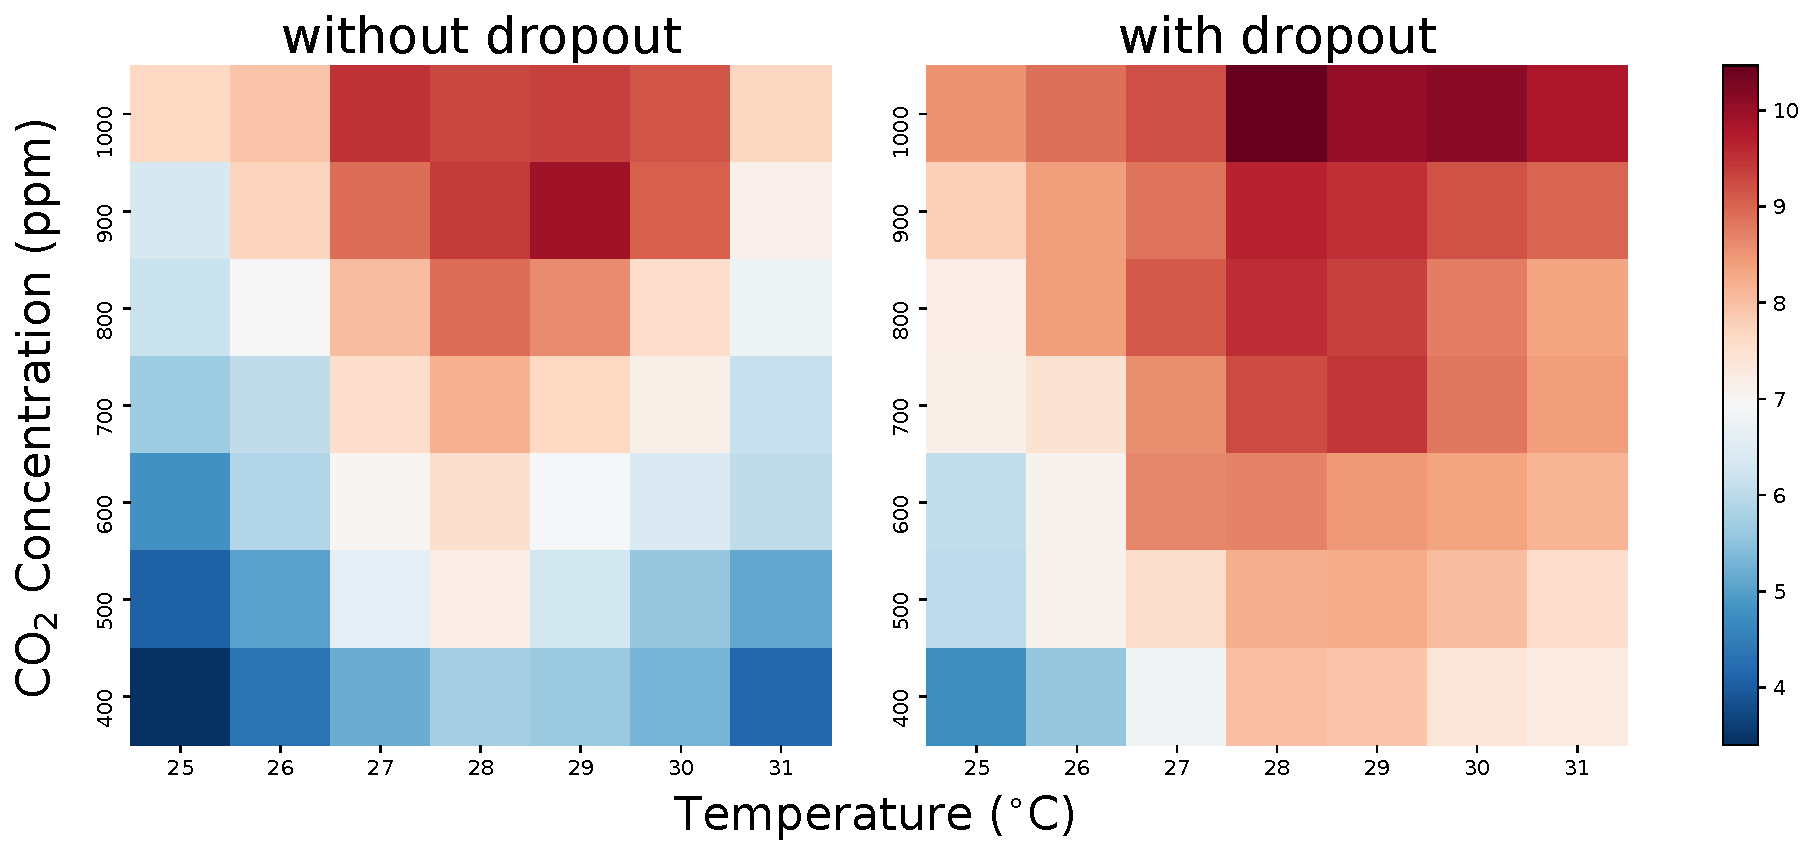
\includegraphics[width=\textwidth]{figures/robustness-heatmap-for-iros.pdf}
\caption{自动温室决策学习算法的鲁棒性实验结果}
\label{fig:robustness}
\end{figure}

为了验证我们算法中样本筛选模块的鲁棒性改进,我们设计了一组抗干扰实验,通过扰动$[25, 31]$区间的温度($^\circ$C)和$[400, 1000]$区间的$CO_2$浓度(ppm)。我们分别测试了有筛选模块和无筛选模块的算法,测试结果如图~\ref{fig:robustness}所示。在上述的热力图中,每个像素代表算法在各个扰动环境中训练相同步数后的预期奖励。其颜色越接近红色意味着奖励越高,反之则代表奖励越低。显然可知,无筛选模块的算法只能在更接近标准区域的小范围内实现正常的预期奖励。相比之下,有筛选模块的算法可以在受干扰较多的地区保持较高的预期奖励,这表明样本样本筛选模块可以显著提高算法的鲁棒性。

为了进一步分析样本筛选模块能带来的好处,我们将外部太阳辐射(Iglob)、温室空气温度(AirT)和温室空气湿度(AirRH)设定为异常参数,它们是作物生长的关键因素。根据这些异常参数,我们在模拟器中测试了我们的算法。在该实验中,我们将作物的新鲜重量和存活率作为指标来评估算法的性能。异常参数的设置和实验结果见表~\ref{tab:exception-test}。

\begin{table}
\centering
\caption{异常参数设置}
\label{tab:exception-test}
\begin{tabular}{c|cc|cc}
\toprule[1pt]
\multirow{2}{*}{\textbf{参数}}                                                 & \multicolumn{2}{c|}{\textbf{作物鲜重}}        & \multicolumn{2}{c}{\textbf{存活率}} \\ \cline{2-5} 
                                                                                    & $p=1$ & $p=0.8$ & $p=1$ & $p=0.8$ \\
\hline
\begin{tabular}[c]{@{}c@{}}$\text{AirT}\in(35,40)$\\\end{tabular} & 38.51                & \textbf{45.24}   & 80.23\%              & \textbf{85.35\%} \\ \hline
\begin{tabular}[c]{@{}c@{}}$\text{AirT}\in(-2,10)$\\ \end{tabular} & 30.31                & \textbf{38.49}   & 63.14\%              & \textbf{72.62\%} \\ \hline
\begin{tabular}[c]{@{}c@{}}$\text{AirRH}=90$\\ \end{tabular}           & 32.69                & \textbf{39.30}   & 68.10\%              & \textbf{74.16\%} \\ \hline
\begin{tabular}[c]{@{}c@{}}$\text{Iglob}=0$\\ \end{tabular}        & 36.76                & \textbf{43.71}   & 76.59\%              & \textbf{82.47\%} \\
\bottomrule[1pt]
\end{tabular}
\end{table}

根据表~\ref{tab:exception-test}中的结果,我们发现,在异常条件下,带有样本筛选模块的算法具有更高的作物新鲜重量和存活率,这代表了更高的安全性,从而验证了样本筛选模块在算法安全性上的提升效果。

\section{本章小结}

本章主要介绍了将所提出的基于模型集成的筛选规划算法应用于真实温室自动化决策控制任务中,进一步验证所提出的算法在苛刻的真实应用场景中的安全性提升效果。本工作具体设计了温室自动化控制策略学习算法,并在仿真模拟器及真实环境中进行了验证实验,样本利用效率和抗环境干扰能力均得以验证,更加充分地证明了所设计的基于模型集成的筛选规划算法能够有效提升强化学习算法的样本利用效率和安全性。